\documentclass[a4paper,twoside, openright,12pt]{report}
\usepackage{psfrag,amsbsy,graphics,float}
\usepackage{graphicx, color} %Deleted [dvips] in front of {graphicx, color} for usage also with PDFLaTex
\usepackage[latin1]{inputenc}
\usepackage{verbatim}
\usepackage{tcolorbox}

% based on the LSR Student Template, last change: 2014-06-05

%_______Kopf- und Fußzeile_______________________________________________________
\usepackage{fancyhdr}
\pagestyle{fancy}
%um Kopf- und Fußzeile bei chapter-Seiten zu reaktivieren
\newcommand{\helv}{%
   \fontfamily{phv}\fontseries{a}\fontsize{9}{11}\selectfont}
\fancypagestyle{plain}{
	\fancyfoot{}% keine Fußzeile
	\fancyhead[RE]{\helv\leftmark}% Rechts auf geraden Seiten=innen; in \leftmark stehen \chapters
	\fancyhead[LO]{\helv\rightmark}% Links auf ungeraden Seiten=außen;in \rightmark stehen \sections
	\fancyhead[RO,LE]{\thepage}}%Rechts auf ungeraden und links auf geraden Seiten
%Kopf- und Fußzeile für alle anderen Seiten
\fancyfoot{}
\fancyhead[RE]{\helv\leftmark}
\fancyhead[LO]{\helv\rightmark}%alt:\fancyhead[LO]{\itshape\rightmark}
\fancyhead[RO,LE]{\thepage}
%________________________________________________________________________________


%_Definieren der Ränder und Längen__________
\setlength{\textwidth}{15cm}
\setlength{\textheight}{22cm}
\setlength{\evensidemargin}{-2mm}
\setlength{\oddsidemargin}{11mm}
\setlength{\headwidth}{15cm}
\setlength{\topmargin}{10mm}
\setlength{\parindent}{0pt} % Kein Einrücken beim Absatz!!
%___________________________________________

%_Hyperref for CC Url__________
\usepackage{hyperref}
%___________________________________________

%_______Title Page__________________________________________
\begin{document}
\pagestyle{empty}
\enlargethispage{4.5cm} %Damit das Titelbild weit genug unten ist!
\begin{center}
\phantom{u}
\vspace{0.5cm}
\Huge{\sc Real-time robot arm control using motor imaginary movements decoded from EEG
	signals}\\
\vspace{1.5cm}
		\large{
			RESEARCH PRACTICE\\%i.e. DIPLOMA THESIS, BACHELOR THESIS, ADVANCED SEMINAR,
			%Intermediate Report\\
			\vspace{0.4cm}
			submitted by\\
			Juri Fedjaev\\
			% if this is a diploma/bachelor/master thesis include the following:
			%\vspace{0.5cm}
			%born on: DD.MM.YYYY\\
			%\vspace{0.5cm}
			%Streetname XX \\
			%Zipcode City \\
			%Tel.: xxx\,xxxxxxxx \\
			\vspace{1.5cm}
			NEUROSCIENTIFIC SYSTEM THEORY\\
			Technische Universit\"at M\"unchen\\
			\vspace{0.3cm}
			Prof. Dr J\"org Conradt\\
		}
\end{center}
\vspace{5.5cm}
\begin{tabular}{ll}
Supervisor: &Dipl.-Ing. Zied Tayed \\
% add the start and intermediate report dates for DA/BA/MA thesis
%Start: & xx.xx.201x  \\
%Intermediate Report: &  xx.xx.201x  \\
Final Submission: &  22.05.2017 \\
\end{tabular}
%____________________________________________________________

\newpage	
\cleardoublepage



\phantom{u}
\phantom{1}\vspace{6cm}
\begin{center}
In your final hardback copy, replace this page with the signed exercise sheet.
\end{center}

\newpage


%_______Abstract_____________________________________________
\topmargin5mm
\textheight220mm
\pagenumbering{arabic}
\phantom{u}
\begin{abstract}
  A short (1--3 paragraphs) summary of the work. Should state the problem, major assumptions, basic idea of solution, results. Avoid non--standard terms and acronyms. The abstract must be able to be read completely on its own, detached from any other work (e.g., in collections of paper abstracts). Don't use references in an abstract.
\end{abstract}
%____________________________________________________________

\newpage

%_______Widmung_______________________________________________
\phantom{u}
\phantom{1}\vspace{6cm}
\begin{center}
%Hier die Widmung oder leer lassen
\end{center}
%_____________________________________________________________



\pagestyle{fancy}

%_________Inhaltsverzeichnis__________________________
\tableofcontents	
%_____________________________________________________32


%_________Einleitung__________________________________
\chapter{Introduction}
People with severe neuromuscular disorders, such as late-stage amyotrophic sclerosis (ALS) and those paralyzed from higher level spinal cord injury are unable to actuate any of their muscles. Communication with the outside world is therefore problematic for the suffering people. Cognitive and sensory body functions, however, are often only minimally affected. Therefore, an electroencephalogram (EEG)-based communication which does not require any neuromuscular control is considered to be particularly helpful to enhance the disabled's quality of life by increasing their independence \cite{birbaumer2006brain}.\\\\
Besides EEG, there are other techniques for monitoring brain activity, such as functional magnetic resonance imaging (fMRI), magnetoencephalography (MEG), positron emission tomography (PET) or single photon emission computer computer tomography (SPECT). The advantages of those methods are a better accuracy and better spatial resolution compared to EEG. However, due to their large size, heavy weight and high price, they are not as suitable for BCI applications as EEG. Furthermore, EEG offers a better temporal resolution, portability and relatively low cost. Recently, low-cost consumer devices came on the market (e.g. EMOTIV EPOC+), which will further push the advancements in the area of EEG-based BCI \cite{sivakamianalysis}. \\\\
In general, the information flow in a BCI follows the following path: signal acquisition, signal (pre)-processing, feature selection and extraction, classification (detection of distinct signal pattern), application interface (e.g. to a robot arm), and feedback (see figure~\ref{fig:bci_control_system}). 

\begin{figure}[htbp]
	\centering
	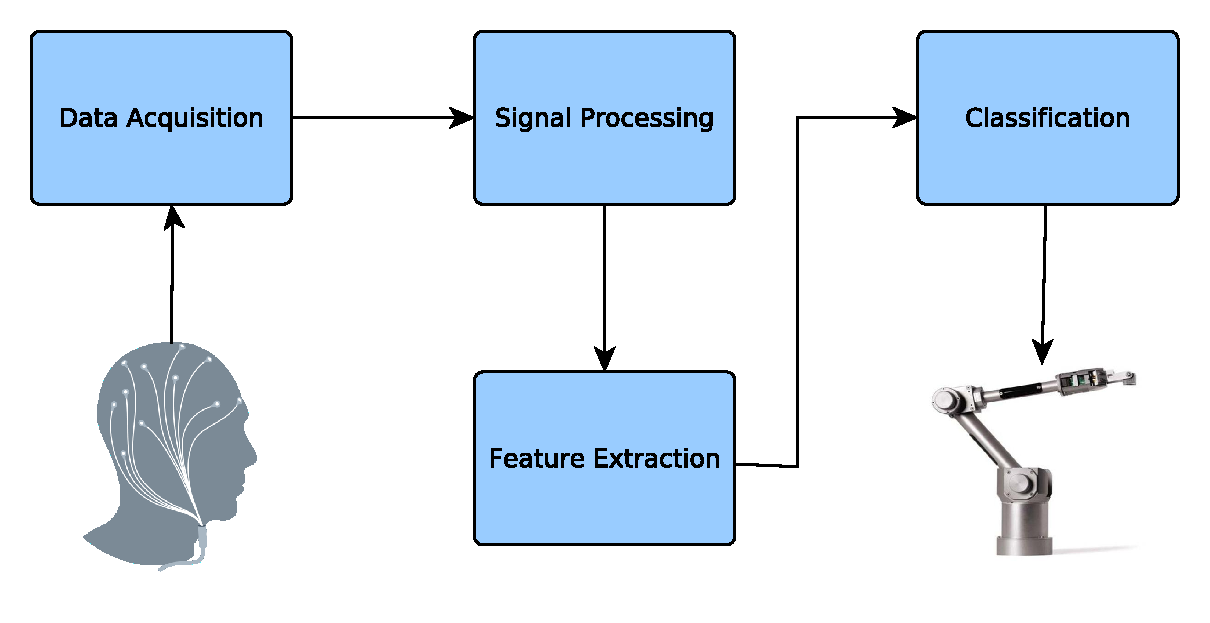
\includegraphics[width=0.8\linewidth]{./gfx/BCI_control_system.pdf}
	\caption{Information flow for a BCI system controlling a robotic arm.}
	\label{fig:bci_control_system}
\end{figure}
For the project of this research practice, the main objective is to implement algorithms similar to those described by Meng and Yong \cite{meng2016noninvasive,yong2015eeg} to discriminate and decode four motor imagery movements (left hand, right hand, both hand imaginary movement and
rest) from EEG signals. Afterwards, the classification has to be used to control a robot arm in a real-time scenario. Motor imagery (MI) is defined as the mental rehearsal or imagination of a physical movement without actually performing it physically \cite{decety1996neurophysiological}. On a neurophysiological level, similar brain regions are activated during motor execution and motor imagery, however, the performance is blocked at a corticospinal level. Studies based on fMRI showed similar activation patterns during motor imagery and actual movement execution \cite{lotze1999activation}. For operating a BCI, motor imagery has proven its capability as an efficient mental strategy. \\\\
Concerning the positioning of the EEG electrodes on the scalp, an internationally recognized method called the 10-20 EEG system is used (see fig.~\ref{fig:10-20-system} for illustration). It was developed to ensure reproducibility by standardizing the electrode positions so that one subject's studies could be compared to each other. The system is based on the relationship between the location of an electrode and the underlying area of cerebral cortex. The "10" and "20" refer to the fact that the actual distances between adjacent electrodes are either 10\% or 20\% of the total front-back or right-left distance of the skull \cite{homan1987cerebral}. Previous studies show that electrode positions C3, Cz and C4 are suitable for recording characteristic motor imagery signals, as they are directly covering part of the sensorimotor area. \\

\begin{figure}[h]
	\centering
	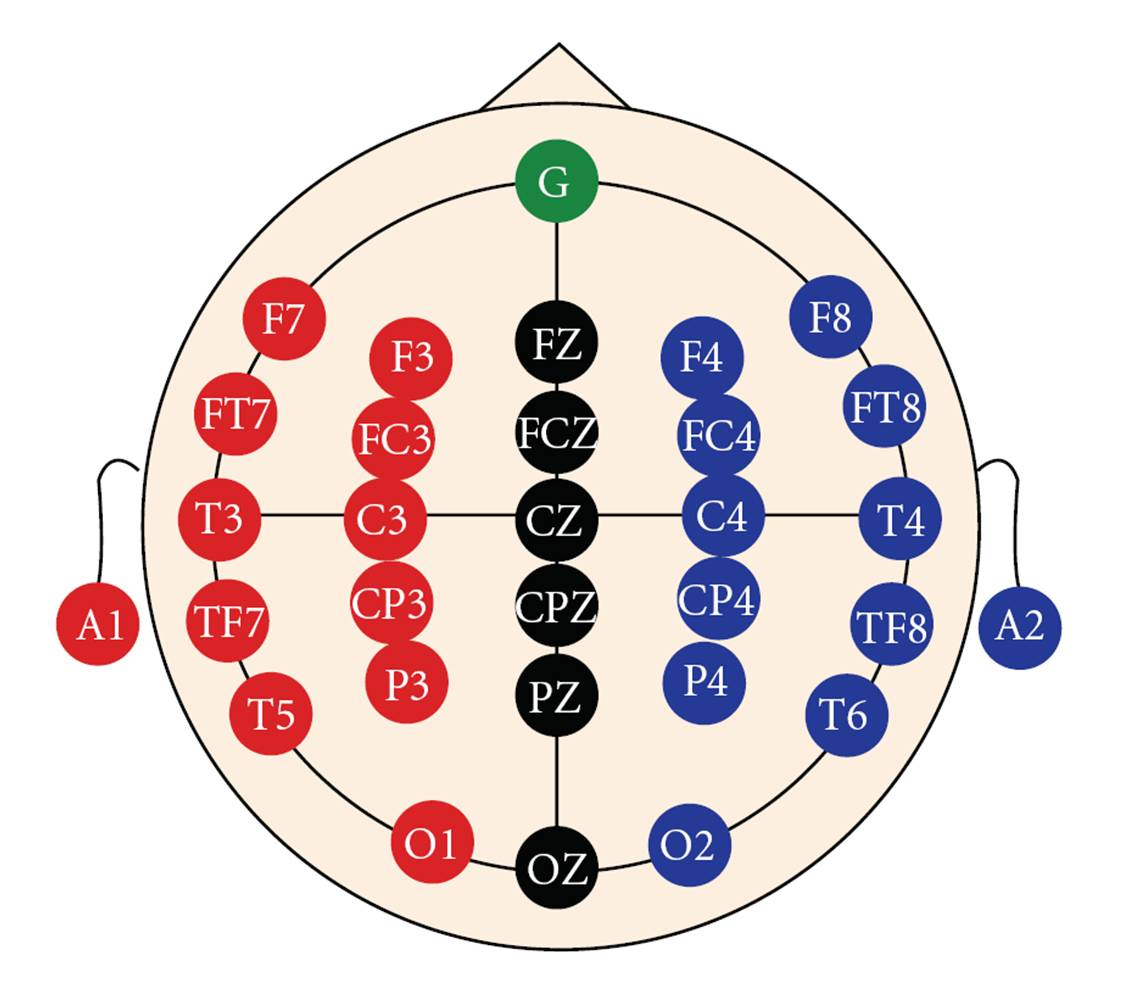
\includegraphics[width=0.5\linewidth]{./gfx/10-20.jpg}
	\caption{International standard 10-20 electrode placement system.}
	\label{fig:10-20-system}
\end{figure}



In the following, first the design and implementation of the BCI project will be discussed. Following that, the accuracies that have been reached will be presented and drawbacks of the approach and possible improvements will be discussed.




%____________________________________________________



%_____Kapitel 2_________________________________
\chapter{Experimental Design and Implementation}
The basic principle on which this BCI project for controlling a robot arm is based on the following idea: First, a training dataset is recorded for subject that wants to execute control commands. Second, that data is used for training a classifier. Subsequently, the trained classifier model is saved and reused for on-line processing the subject's EEG data, enabling real-time robot control. In order to accelerate that procedure and minimize time constraints, there exist several frameworks for BCI applications. To name some of the most commonly used:
\begin{itemize}
	\item BCILAB\\
	$\circ$  "Open-source MATLAB-based toolbox built to address the need for BCI methods development and testing by providing an organized collection of over 100 pre-implemented methods and method variants, an easily extensible framework for the rapid prototyping of new methods, and a highly automated framework for systematic testing and evaluation of new implementations" \cite{kothe2013bcilab}.
	\item OpenVibe\\
	$\circ$ "OpenViBE is a software for real-time neurosciences (that is, for real-time processing of brain signals). It can be used to acquire, filter, process, classify and visualize brain signals in real time. OpenViBE is free and open source software. It works on Windows and Linux operating systems" \cite{journals/presence/RenardLGCMDBL10}.
	\item BCI2000\\
	$\circ$ "BCI2000 is a software suite for brain-computer interface research. It is commonly used for data acquisition, stimulus presentation, and brain monitoring applications. BCI2000 supports a variety of data acquisition systems, brain signals, and study/feedback paradigms. [...] BCI2000 is available free of charge for research and education purposes" \cite{schalk2010practical}.
\end{itemize}

\section{First approach: OpenVibe and Emotiv EPOC+}
As previously mentioned, using an existing software framework accelerates development enormously. Therefore, the first approach was to use OpenVibe to implement the BCI system. This was possible because the EEG system for signal acquisition that was available in the beginning of the project was the Emotiv EPOC+. The EPOC+ is a wireless, 14 channel-device with a sampling rate of $128$ Hz (see fig.~\ref*{fig:openvibe_blocks} on the right-hand side). Its electrodes cover many of the electrode positions as proposed by the 10-20 system (see above), thus also the area near the sensorimotor cortex at C3 / C4 locations. Furthermore, Emotiv offers driver support for its use with OpenVibe.\\
OpenVibe's programming paradigm is based on building blocks representing individual signal processing algorithms which can be easily connected to each other. Using Python and/or C++, it is also possible to build new blocks with user specific algorithms (see fig.~\ref{fig:openvibe_blocks} on the left-hand side for an illustration).
\begin{figure}[tbph!]
\centering
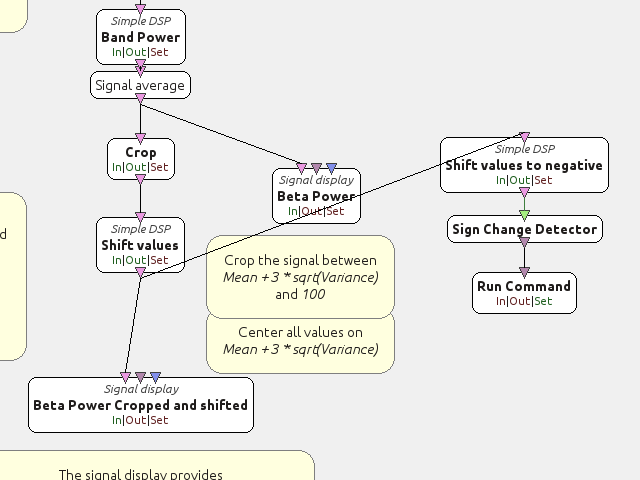
\includegraphics[width=0.6\linewidth]{gfx/openvibe_blocks}
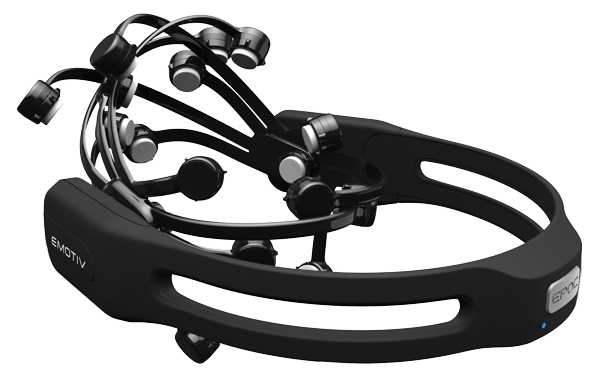
\includegraphics[width=0.39\linewidth]{gfx/emotiv_epoc}
\caption{Left: Example for the work flow in OpenVibe using algorithmic building block. Right: The Emotiv EPOC+ headset for signal acquisition.}
\label{fig:openvibe_blocks}
\end{figure}
The interface to OpenVibe is the so-called \textit{OpenVibe Acquisition Server}. For accessing the raw signals of the EPOC+, a premium software development kit (SDK) is needed. However, there are issues trying to connect the EPOC+ with the OpenVibe aquisition server. In fact, the connection succeeds but stops working when starting the acquisition (see fig.~\ref{fig:epoc_error}).
 
\begin{figure}[h]
	\centering
	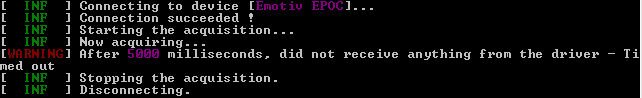
\includegraphics[width=0.8\linewidth]{./gfx/epoc_errorcode}
	\caption{Error encountered when trying to connect the Emotiv EPOC+ with OpenVibe Acquisition Server.}
	\label{fig:epoc_error}
\end{figure}

Two similar headsets with the official premium SDK were tested without success. Emokit reverse-engineering drivers written in Python (found on GitHub) were able to access some of the data. However, the electrode and quality indicators were disturbed by a strong jitter in the data. An Emotiv EPOC+ headset with an older version number was working without any problems, but was unfortunately available only briefly for testing purposes and not for the BCI project. Therefore, it is assumed that there were some changes done on firmware level by the manufacturer. In the end, the approach using an Emotiv EPOC+ in connection with OpenVibe was abandoned due to the previously described problems. The alternative solution will be explained in the following section.

\section{Second Approach - Biopac MP36}
Following the difficulties using the Emotiv headset, alternative hardware for EEG signal acquisition was needed. Fortunately, NST has two Biopac MP36 systems available. The Biopac MP36 is a biosignal acquisition device specifically developed for undergraduate students studying physiology. It is distributed as a complete solution called \textit{Biopac Student Lab} (BSL). The BSL system integrates hardware, software and curriculum materials including over sixty experiments that students use to study the cardiovascular system, muscles, pulmonary function, autonomic nervous system, and the brain \cite{biopac_general}.\\
The MP36 has four analog input channels, each with separate ground and reference electrodes. It has an A/D sampling resolution of 24-Bit and a maximum sampling rate of $100$ kHz per channel, see figure~\ref*{fig:biopac}.

\begin{figure}[htbp!]
	\centering
	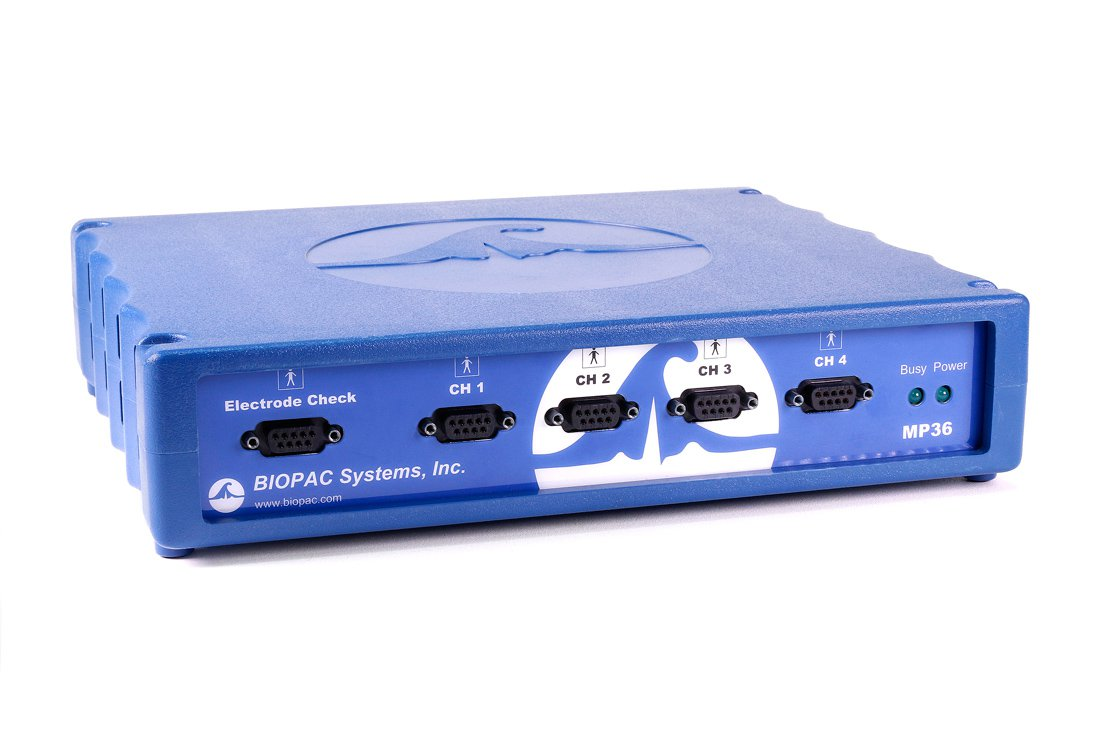
\includegraphics[width=0.32\linewidth]{./gfx/mp36}
	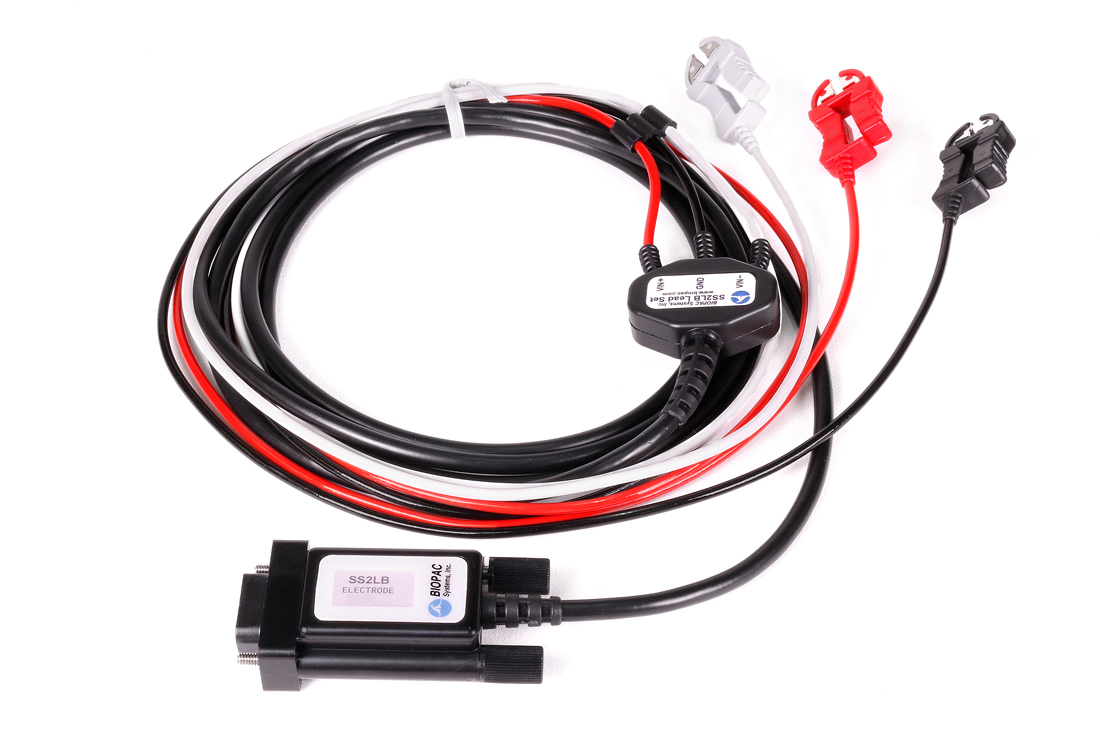
\includegraphics[width=0.32\linewidth]{./gfx/biopac_cable}
	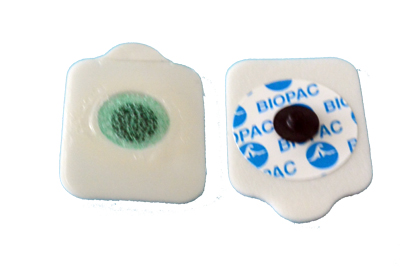
\includegraphics[width=0.32\linewidth]{./gfx/biopac_electrodes}
	\caption{Left: Biopac MP36 data acquisition unit. Middle: Biopac electrode connection cable with separate reference and ground per channel. Right: Disposable Biopac electrodes. }
	\label{fig:biopac}
\end{figure} 

As the Biopac system is supposed to be used with the proprietary Biopac Student Lab software, there is no BCI software available that supports the MP36 acquisition device natively. However, Biopac provides a hardware API (BHAPI) for developers. The BHAPI enables the user to acquire raw data, set sampling rate, triggers, get the status of the MP36 device as well as some other features. The implementation of these functions is compiled into a Windows 32-Bit DLL (dynamic link library) called \texttt{mpdev.dll} (see fig.~\ref*{fig:bhapi}). The interface is documented in C/C++, but any programming language that is able to utilize Windows 32-bit DLLs should be able to access the BIOPAC Hardware API. Due to personal preferences Matlab is used.

\begin{figure}[htpb!]
	\centering
	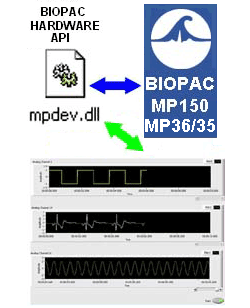
\includegraphics[width=0.3\linewidth]{./gfx/bhapi.png}
	\caption{Illustration of the Biopac hardware API as an interface to external programming languages or software (here: LabView). }
	\label{fig:bhapi}
\end{figure}

\subsection{Data Acquisition}
In order to train the classifier model, training data is necessary. Therefore, a cue-based experimental paradigm was used. The participants of the data recording sessions were shown visual cues in form of left or right arrows at distinct points in time for the onset of left or right arm motor imagery of movements (see figure~\ref{fig:exp_design}), representing the two classes. One recording sessions consisted of 40 or 50 trials, 20 or 25 trials, respectively, for each side (left, right). One trial has a total duration of 8 seconds, with cue onset on second 3 for a duration of 2 seconds. During cue display, the participant is supposed to maintain the motor imagery accordingly (see figure~\ref{fig:exp_design} for illustration).\\
For the training sessions, a Matlab function \texttt{recordMotorImageryData(numTrials, nCh, cueOn)} has been written. It takes as input arguments the desired number of trials (\texttt{numTrials}), the number of channels used for recording (\texttt{nCh}), and whether a cue shall be displayed or not (\texttt{cueOn}). If a cue is not desired, the function will plot a graph of the EEG. 
\begin{figure}[htbp!]
	\centering
	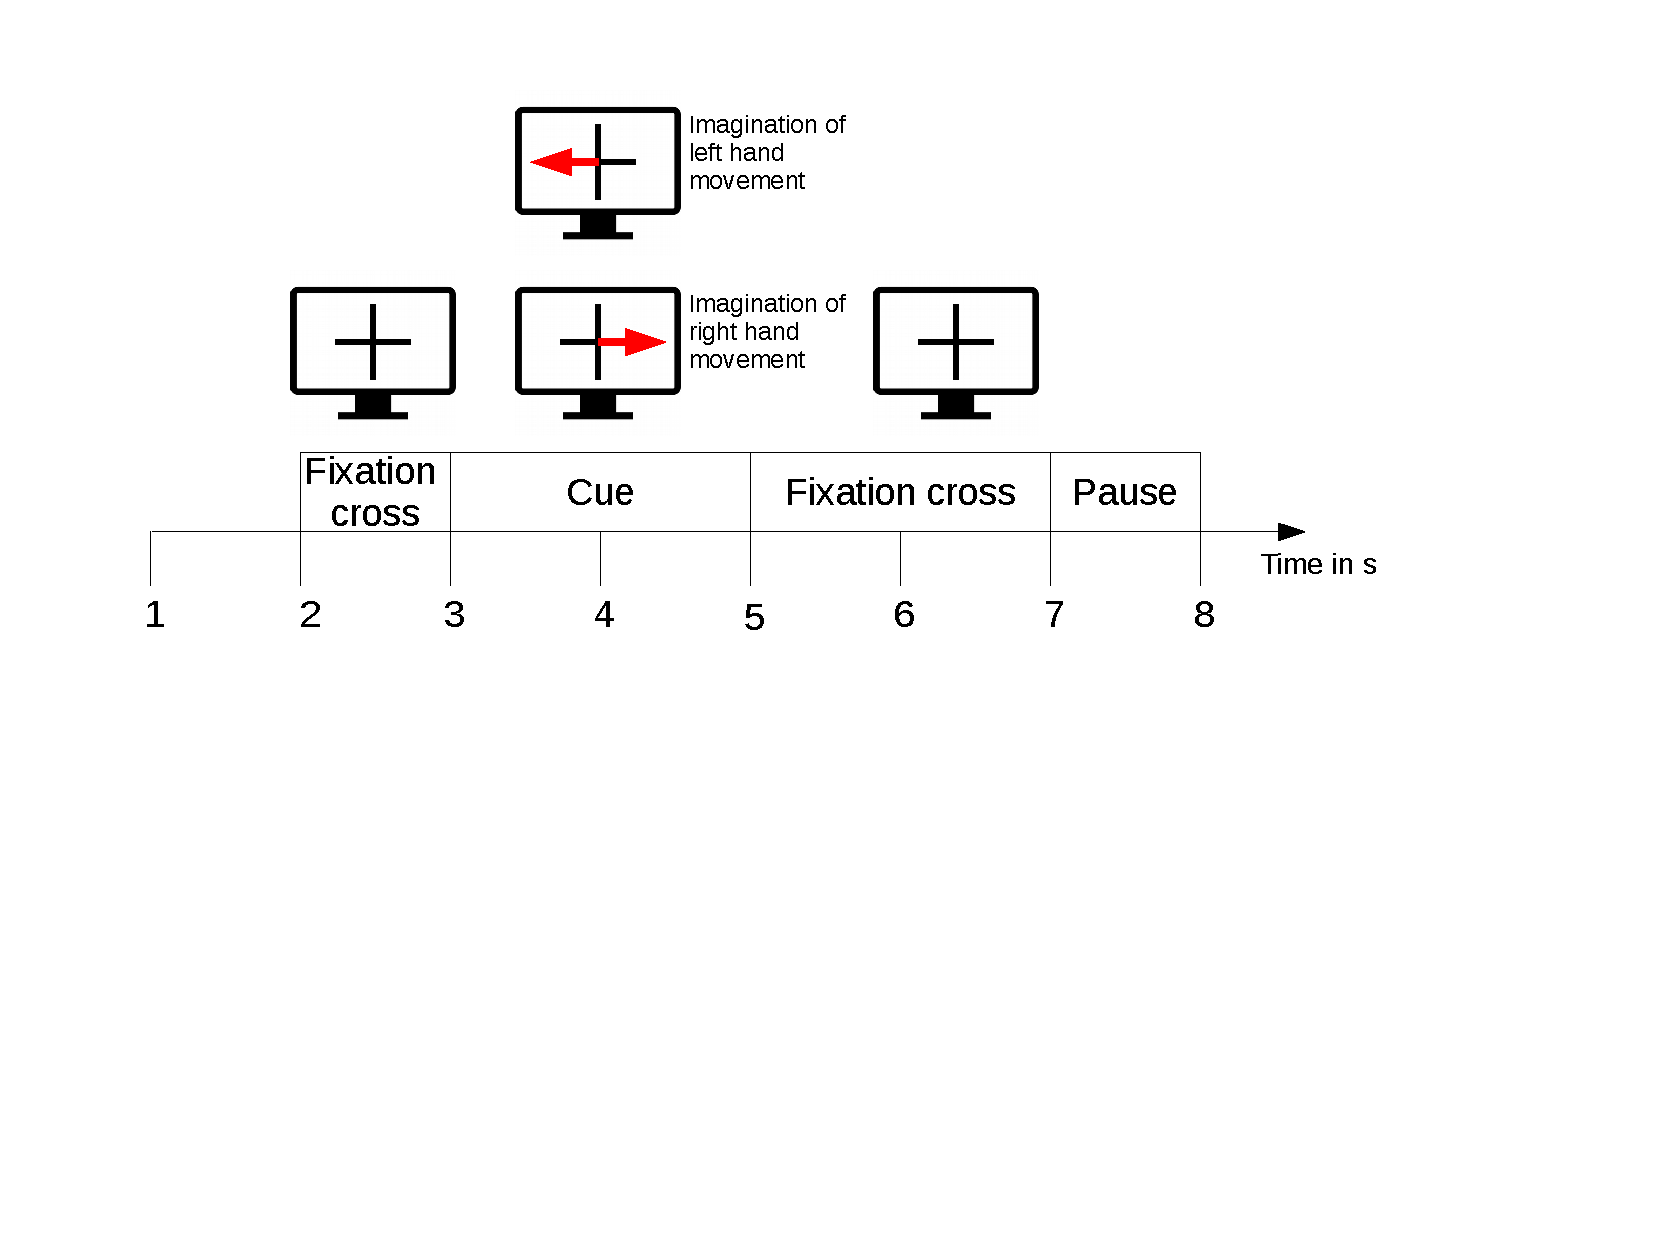
\includegraphics[width=1\linewidth]{./gfx/exp_design}
	\caption{Timing of the movement imagery task. Visual cue stimulus in form of left/right arrows between 3 and 5 seconds instructs the participant o imagine the desired movement (of left/right arm, respectively).}
	\label{fig:exp_design}
\end{figure}
\paragraph{Launching data acquisition:} In order to start the MP36 acquisition device, an interface to Matlab was written, namely the function \texttt{startAcquisition(dothdir, libname,mptype, mpmethod, sn, duration)}. It takes as inputs the path to the C/C++ header file \texttt{mpdev.h} (\texttt{dothdir}), the name of the Biopac API DLL file (\texttt{libname}), the type of Biopac device (\texttt{mptype}, has value '\texttt{103}' for MP36), the connection method \texttt{mpmethod} (has value '\texttt{10} for USB connection), the serial number of the Biopac device \texttt{sn} (can be put to '\texttt{auto}', if only a single Biopac device is connected to the computer), and finally the duration of data acquisition in seconds \texttt{duration}. 

\paragraph{Cue display:} For cue display, another Matlab function \texttt{launchCueExp(DURATION, T\_BLANK, T\_CUE\_ON, T\_CUE, T\_PERIOD)} has been written. By modifying its input parameters, individual visual cue timings may be re-used for future experiments at NST. The inputs are the total experiment duration in seconds \texttt{DURATION}, the fixation cross onset \texttt{T\_BLANK}, the cue onset time \texttt{T\_CUE\_ON}, the duration of cue display \texttt{T\_CUE}, and the period length for one trial \texttt{T\_PERIOD}. For illustration of the parameters see figure~\ref{fig:exp_design}.

\paragraph{Data Format:}

\subsubsection*{Electrode positioning}
The electrode positioning on the scalp is a crucial part of BCI design. As mentioned before, electrode positions on C3, Cz and C4 are desired for motor imagery classification tasks. Therefore, each of the bipolar electrode pairs are positioned accordingly on those positions (see figure~\ref{fig:elec_pos} in the middle for illustration). The ground electrodes may be positioned on the mastoid parts of the temporal bone, right behind the ears (see figure~\ref{fig:elec_pos} on the left for illustration). As the electrodes used with the Biopac device are dry electrodes that are more suitable for EMG recordings, great caution must be exercised while placing them. Participants with thick hair may be a problem due to low signal-to-noise ratio (SNR) and high impedance. The subject's hair should be gently moved to the sides, so that the electrodes touch the scalp. After placement, the the electrodes should be pressed onto the scalp with minor force for roughly one minute each. Then, bandages were wrapped around the subjects head to fixate the electrodes. The impedance for the electrodes should ideally be lower than $10$ k$\Omega$, which can be checked using the "\textit{Impedance Check}" port on the Biopac device. A value under $50$ k$\Omega$, however, was accepted during recordings, as it was hard to achieve a lower values.\\ 
\begin{figure}[htbp!]
	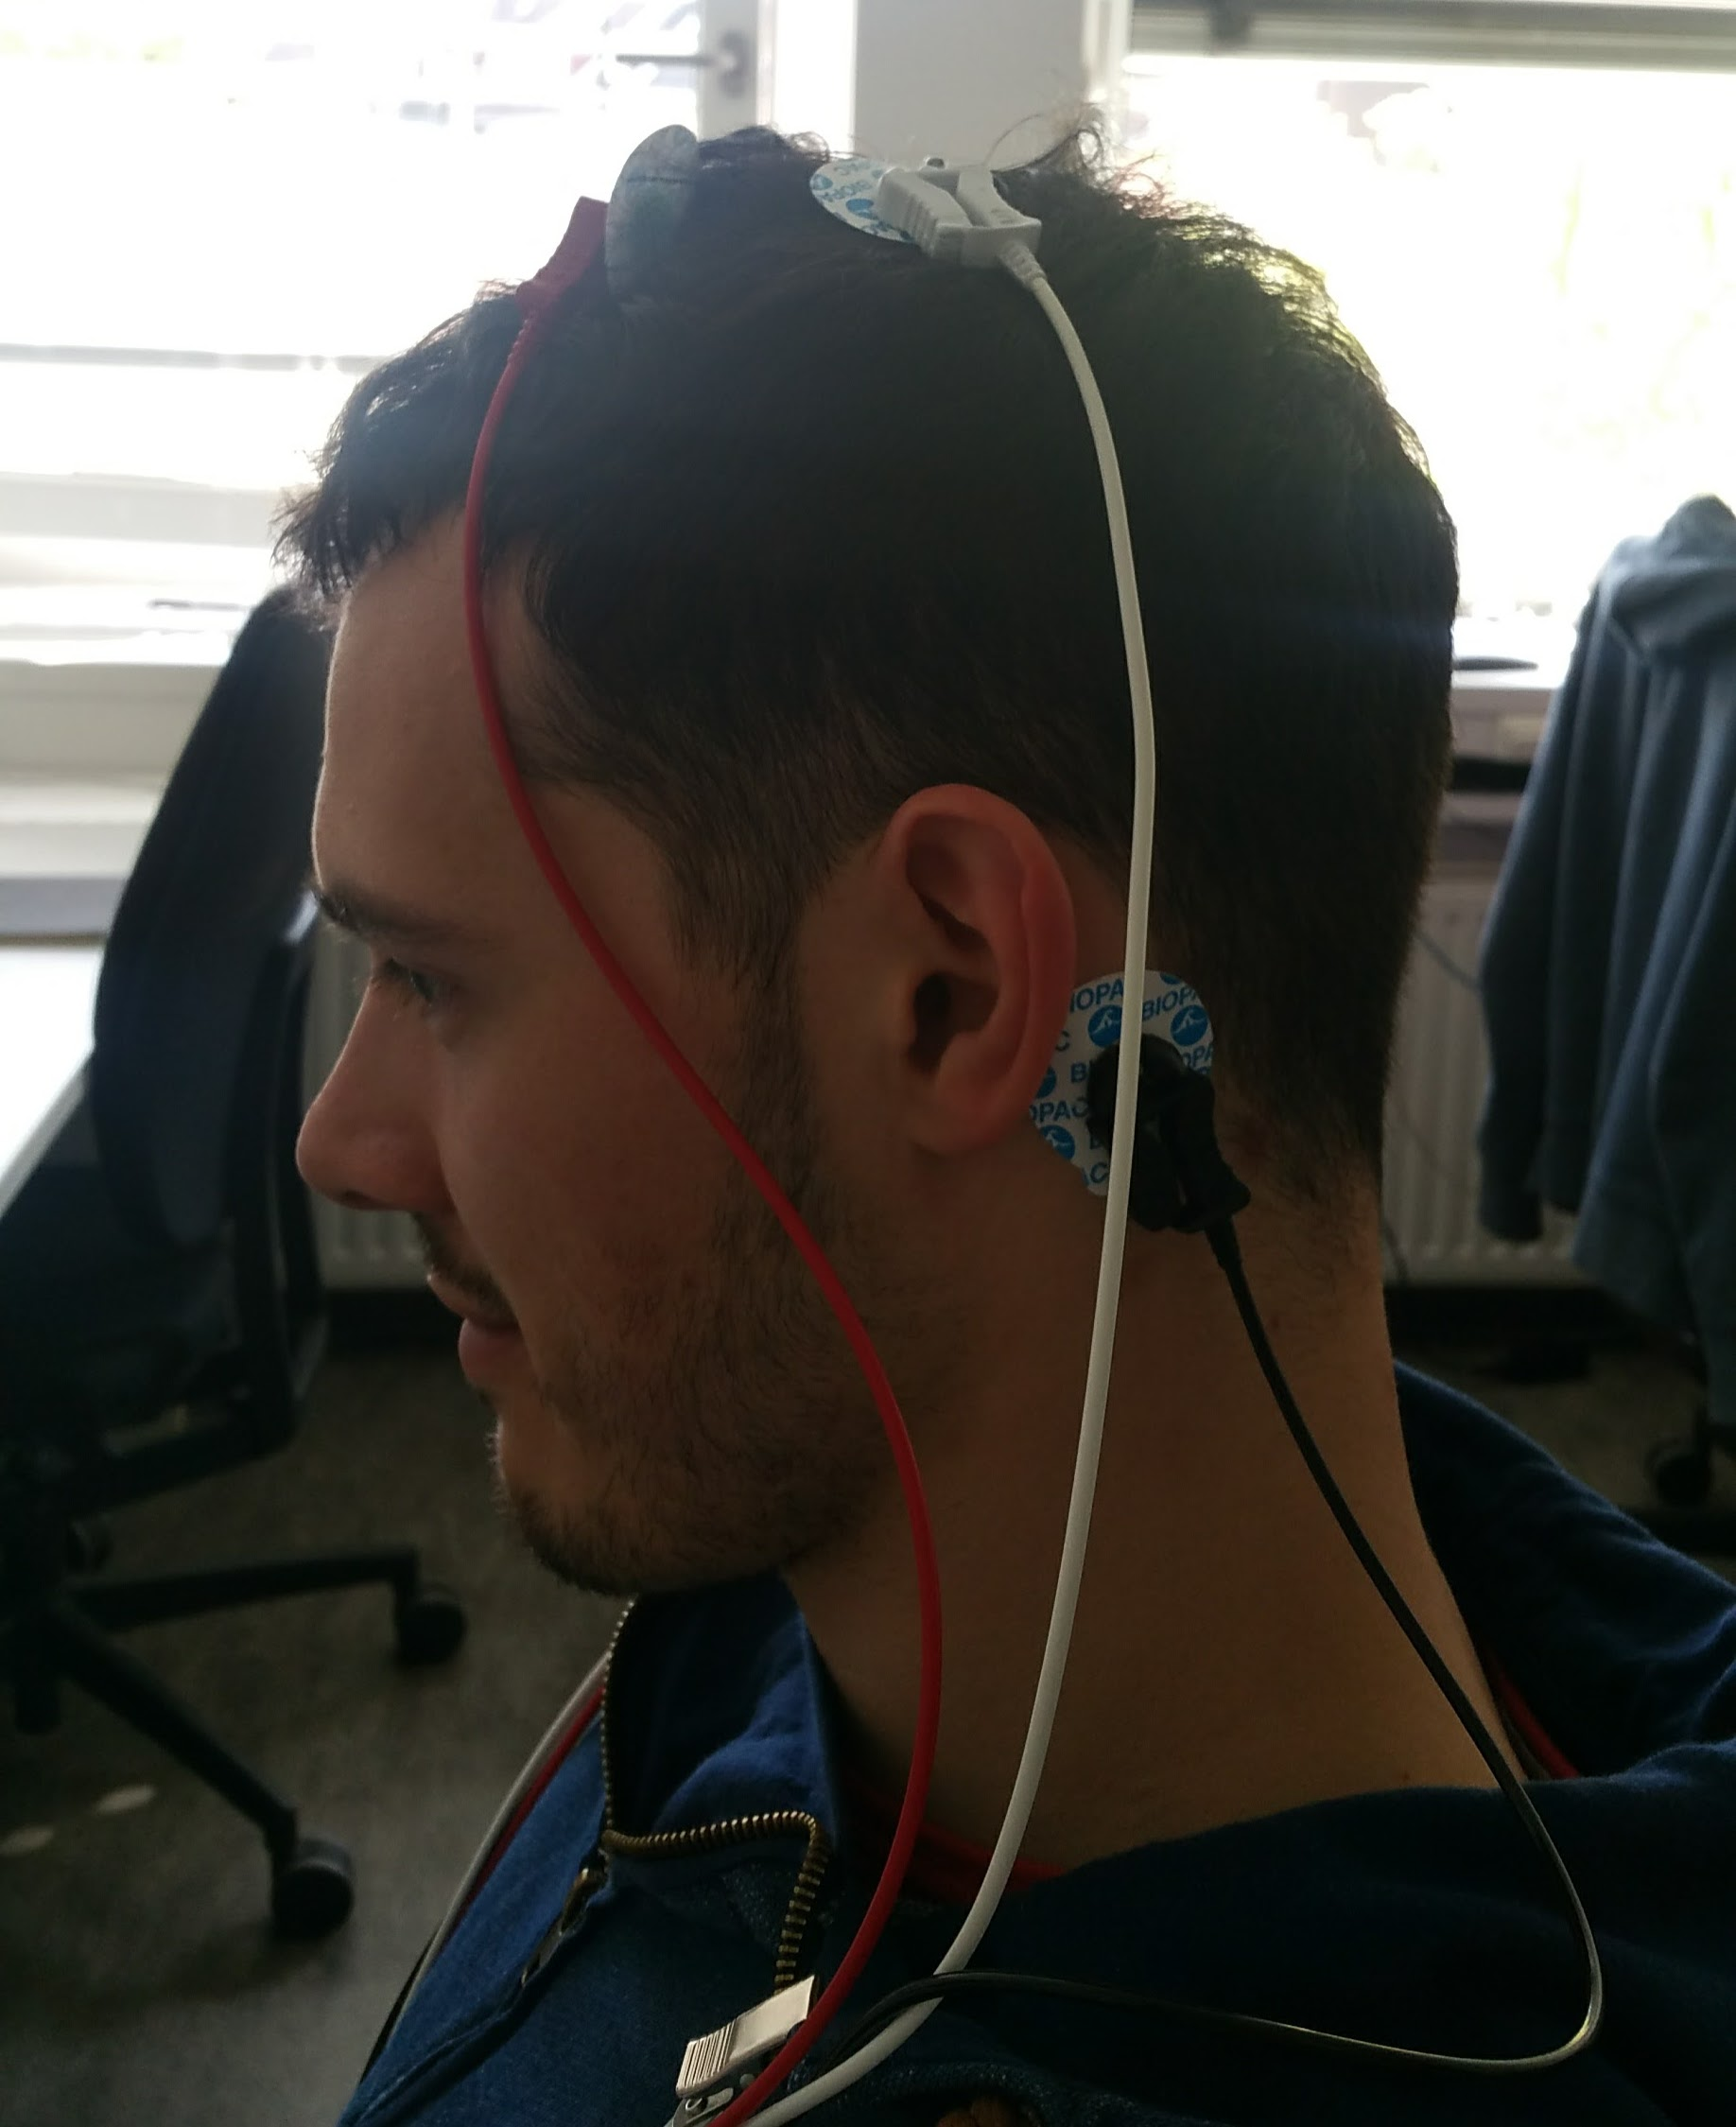
\includegraphics[width=0.32\linewidth]{./gfx/alex_side}
	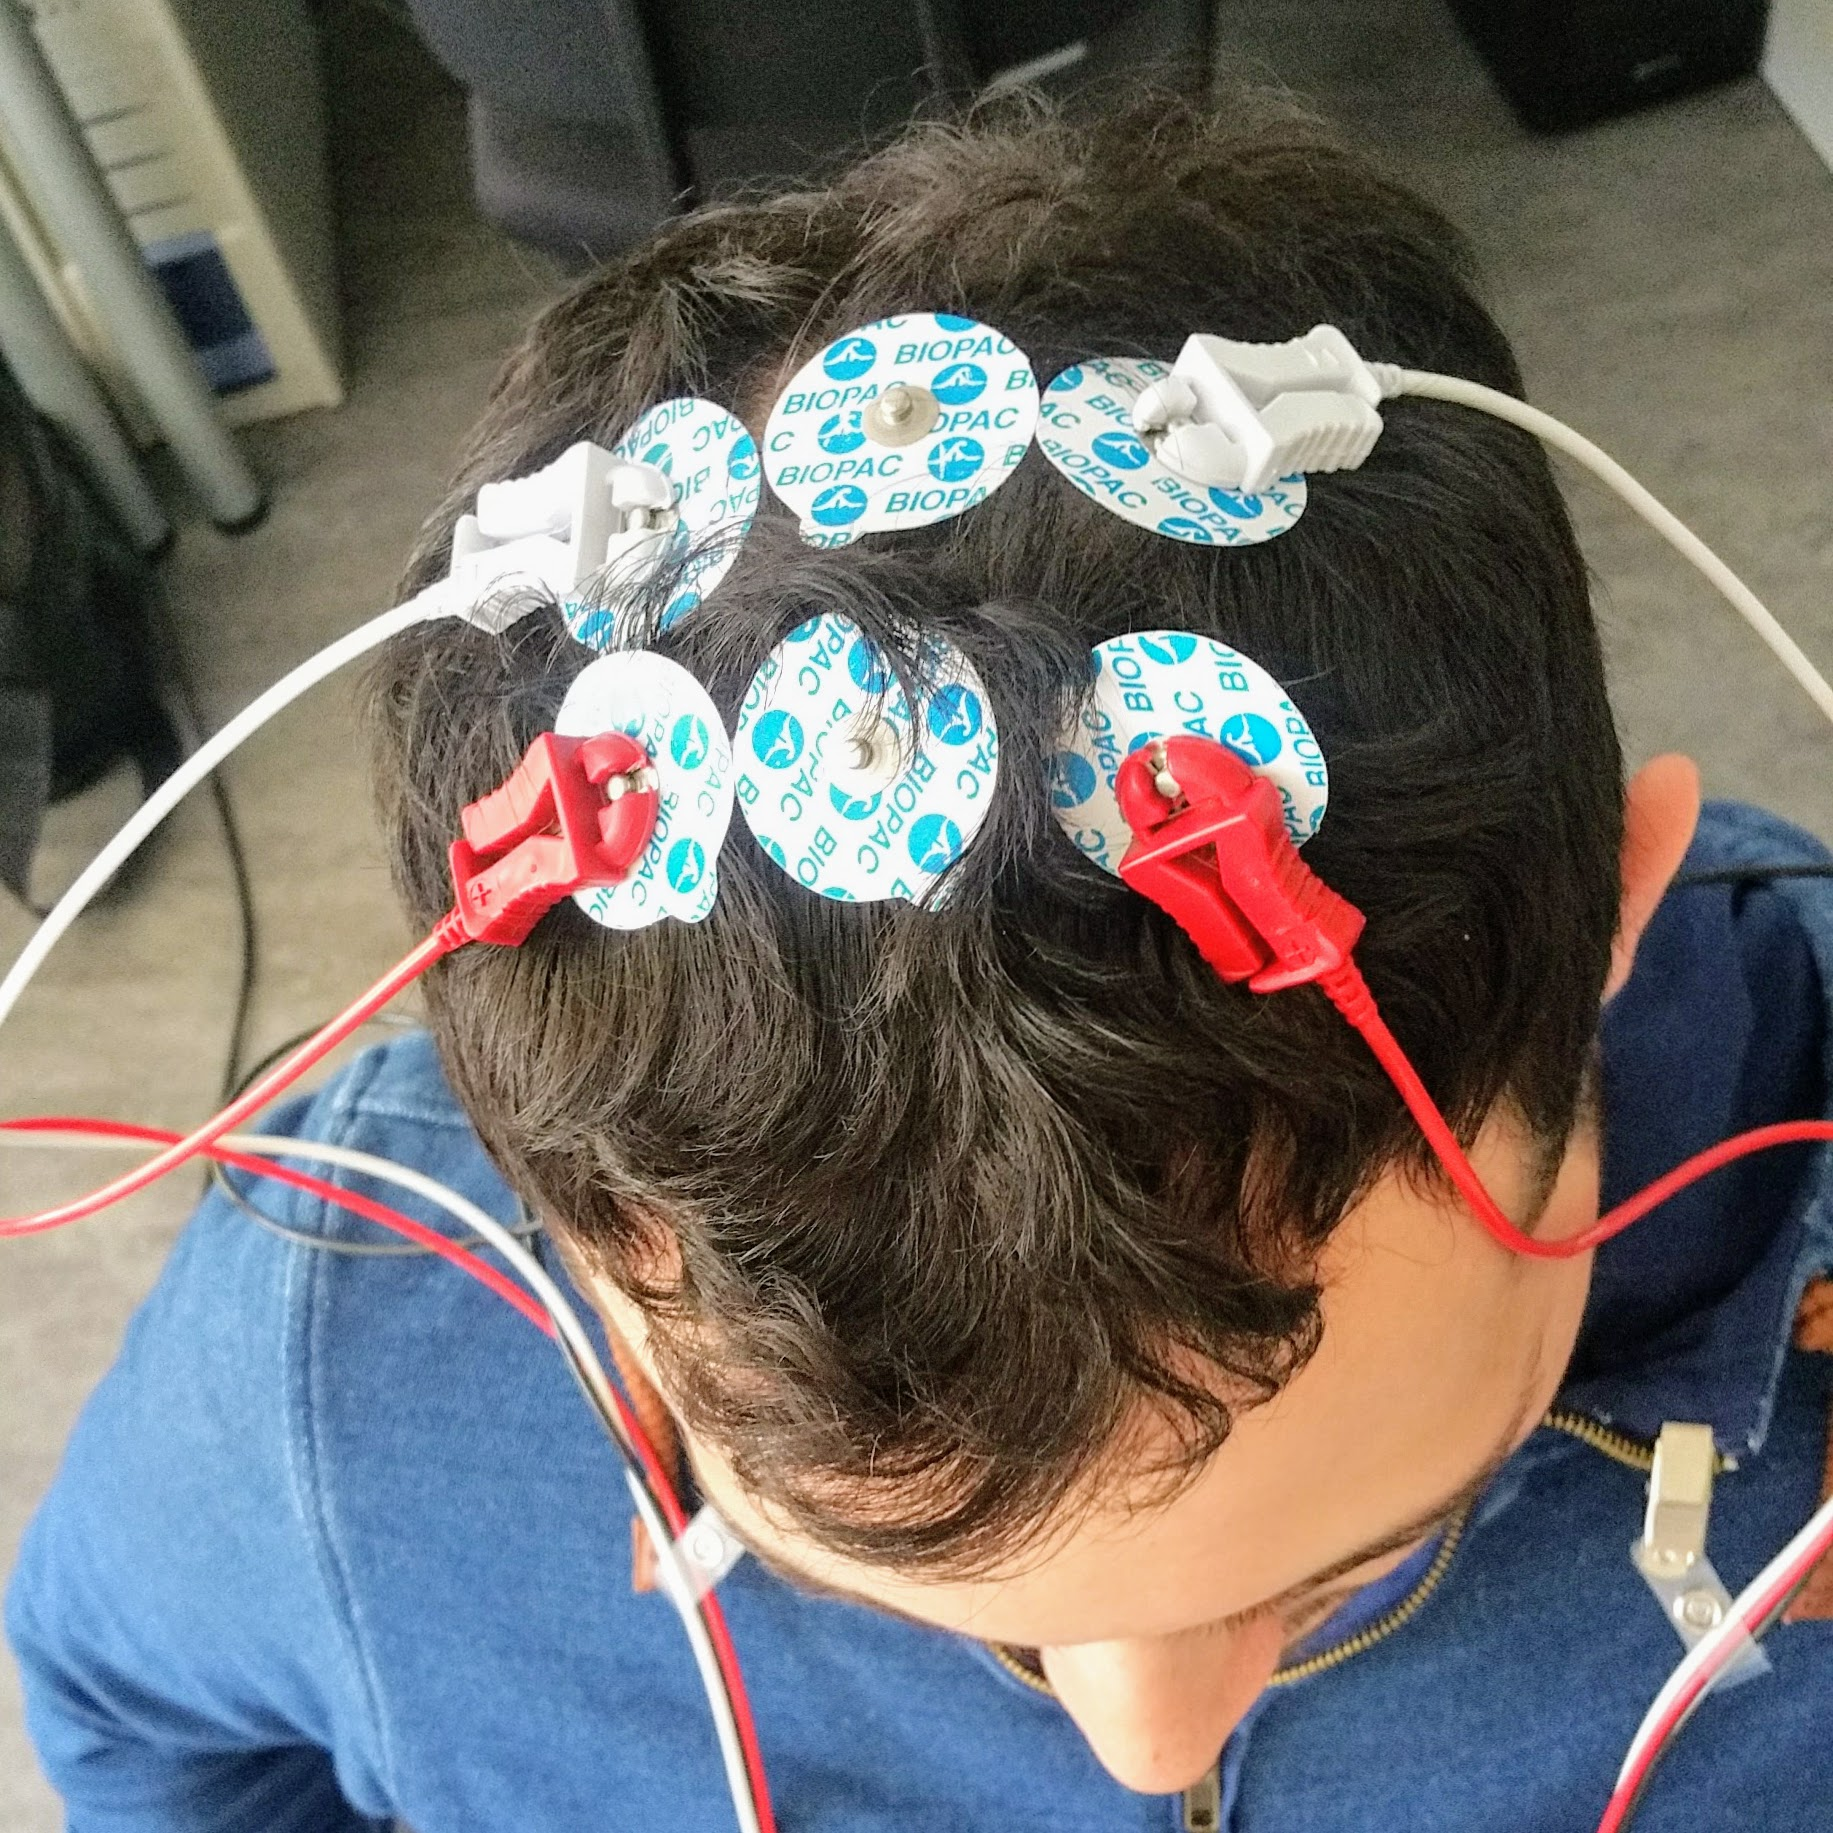
\includegraphics[width=0.32\linewidth]{./gfx/alex_top}
	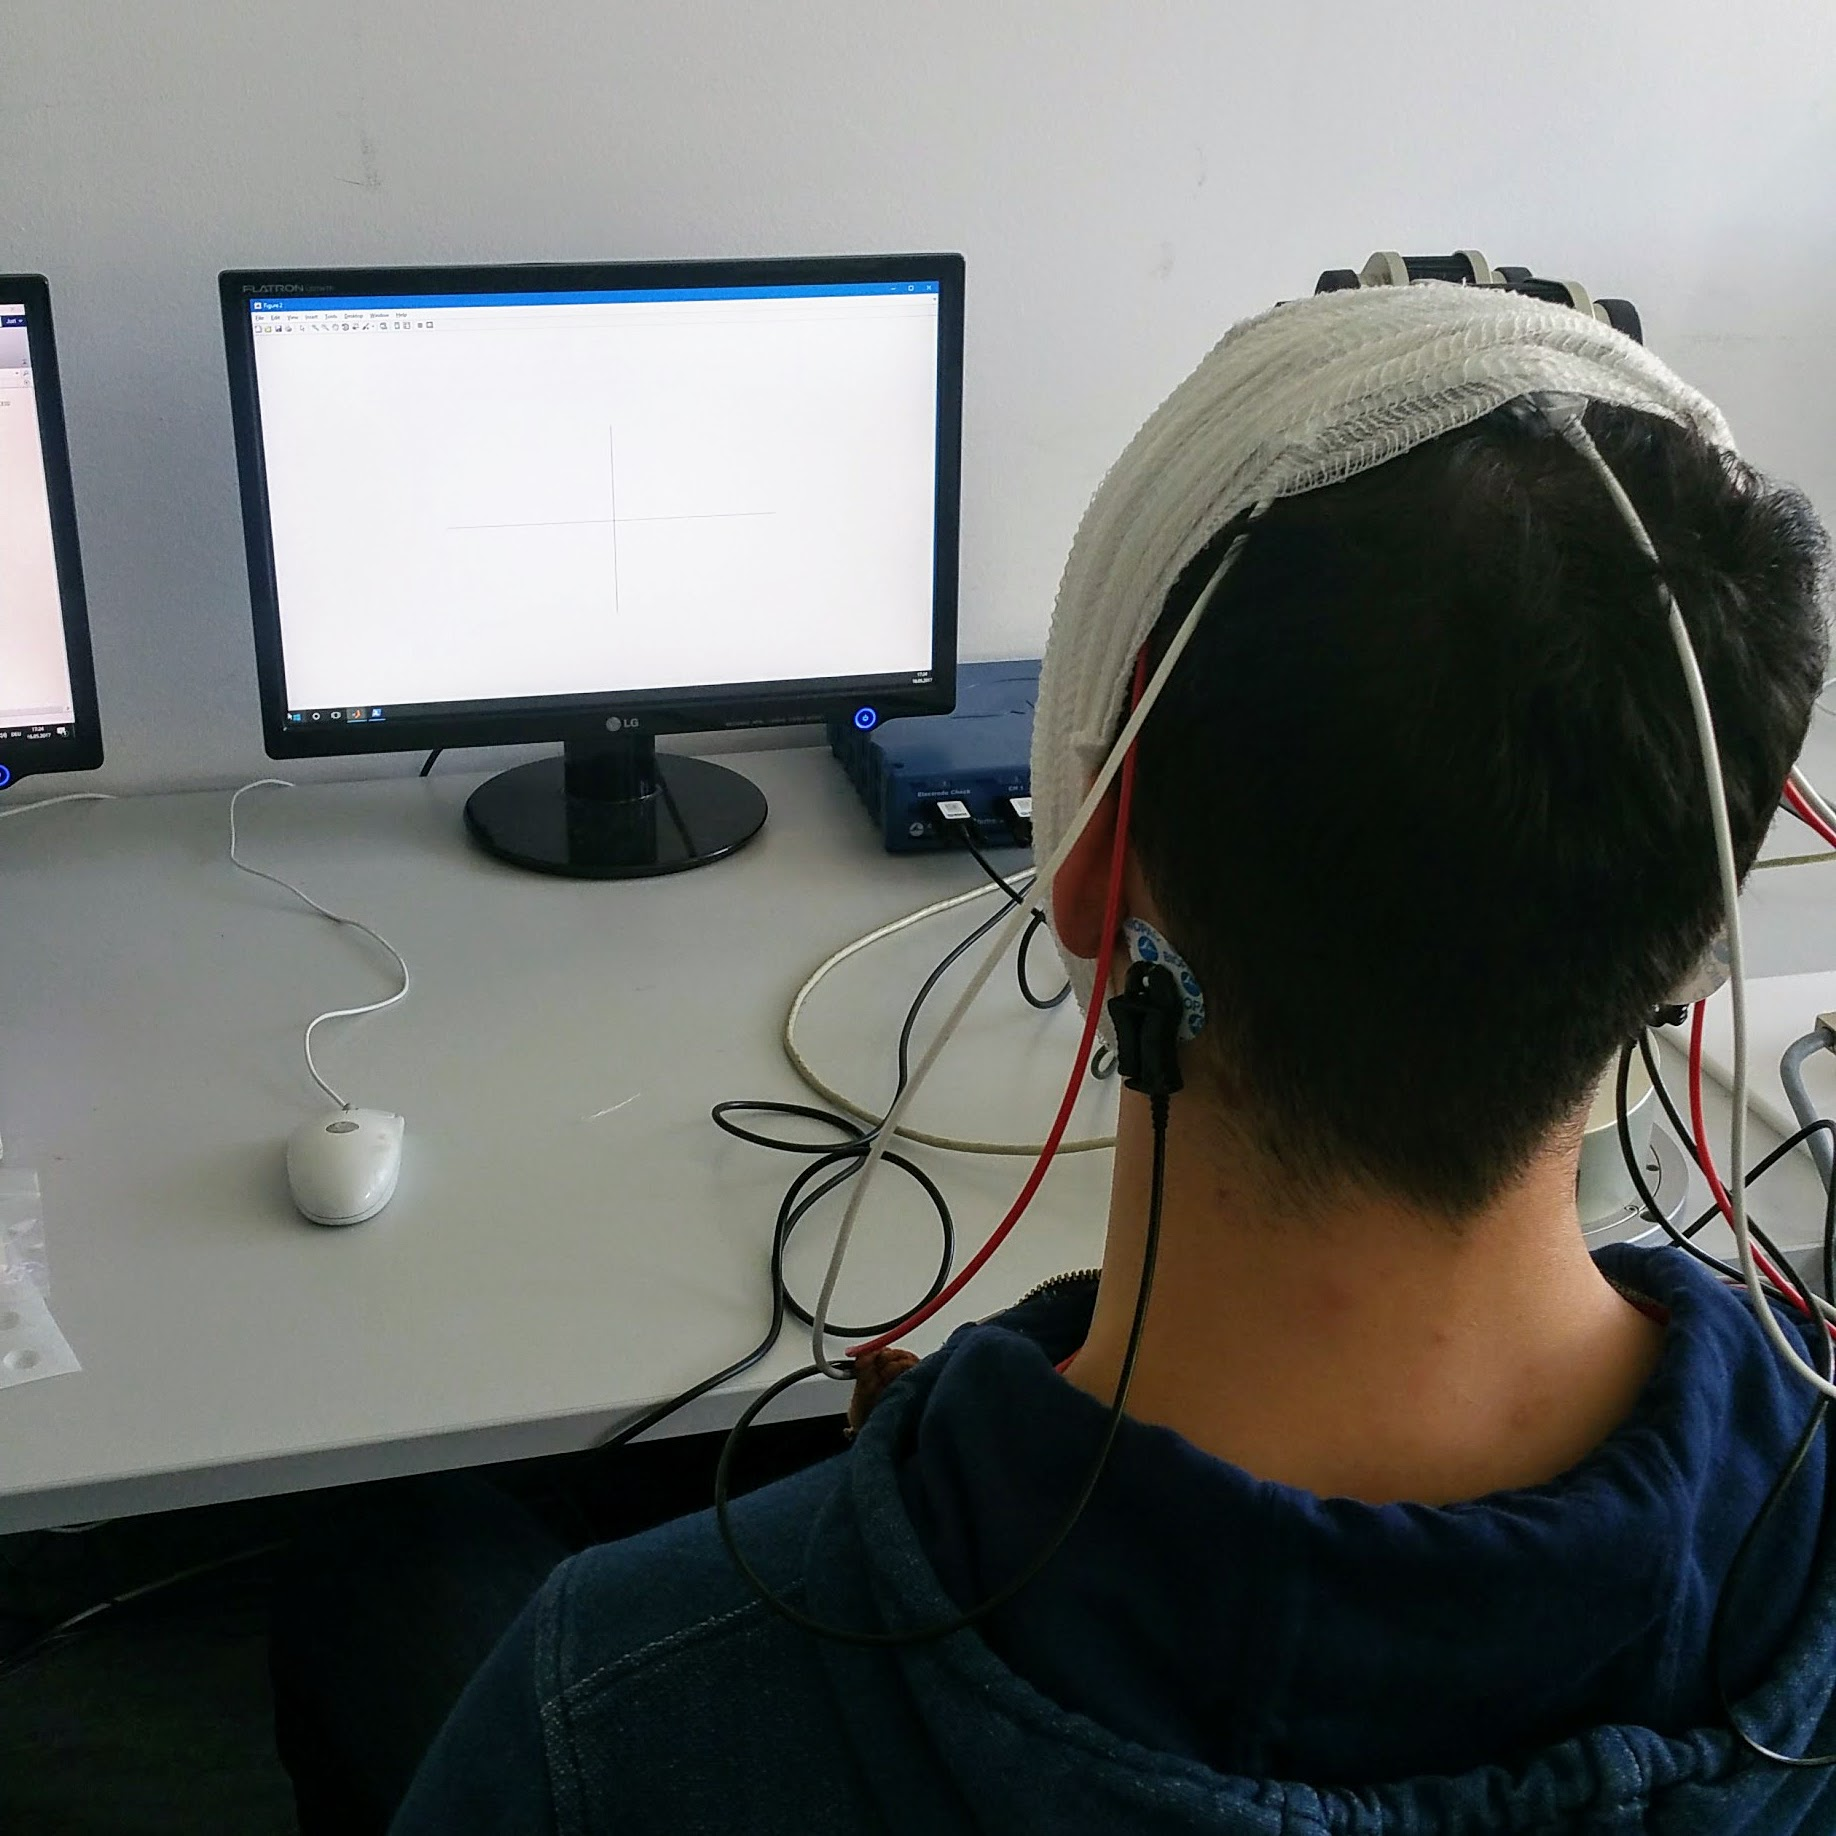
\includegraphics[width=0.32\linewidth]{./gfx/alex_back}
	\caption{Left: Electrodes on subjects scalp as seen from the left-hand side with ground electrode on the mastoid part of the temporal bone. Middle: View from the top showing C3, Cz and C4 electrode positions (l.t.r.) using bipolar derivation. Right: Subject's view and position for the recording session.}
	\label{fig:elec_pos}
\end{figure}
As a side note, the recording setup with the Biopac device is very uncomfortable for the participant and was unsustainable for longer periods of time ($> 15$ min). After the recording, the removal of the electrodes is tedious and painful because the adhesive that sticks strongly onto the hair. 

\subsection{Signal pre-processing}
As the data is ...


\begin{figure}[htbp!]
	\centering
	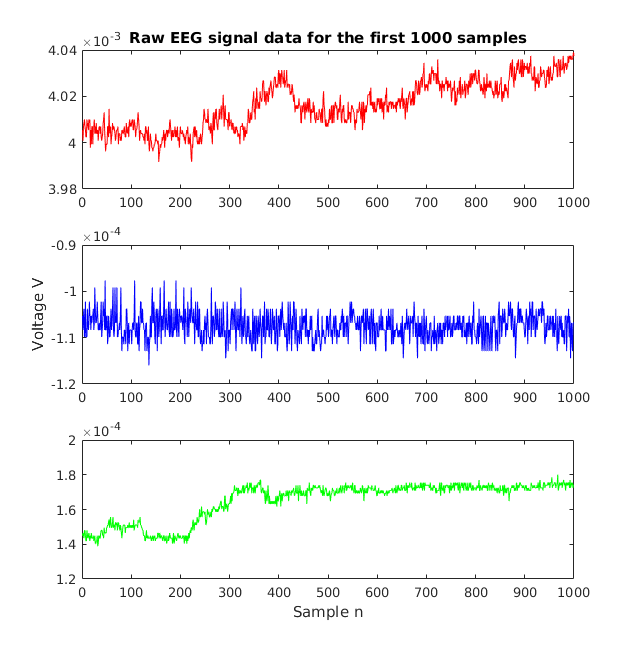
\includegraphics[width=0.49\linewidth]{./gfx/raw}
	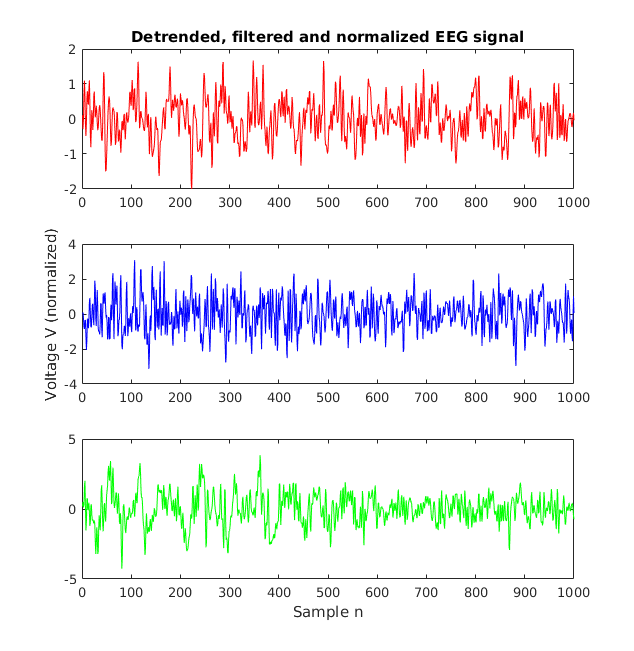
\includegraphics[width=0.49\linewidth]{./gfx/filtered}
	\caption{Left: Raw signals from channels 1, 2 and 3. Right: Removed baseline drift, bandpass filtered and normalized signals from channels 1, 2 and 3.}
	\label{fig:signals}
\end{figure}


\section{Experimental Results}

\begin{itemize}
	\item reached accuracies of SVM
	\item how to ensure that recording is successful  
	\item ...
\end{itemize}s


\section{Discussion}
\begin{itemize}
	\item how to improve classification accuracy
	\subitem improve feature extraction, e.g. use ERD / ERS on $\alpha$- / $\beta$-bands 
	\item use different classifier 
	\subitem ANN or SNN would be interesting to see. See paper xy for examples
	\subitem Convolutional NN or recurrent deep NN could significantly improve classification accuracy and therefore enable the system for a multiclass (more than two for instance) classification 
\end{itemize}


Discuss and explain your results. Show how they support your thesis (or, if they don't, give a convincing explanation). It is important to separate objective facts clearly from their discussion (which is bound to contain subjective opinion). If the reader doesn't understand your results, reconsider if you have managed to extract the core information and explain it in a straightforward way.

%_______________________________________________



%_____Zusammenfassung, Ausblick_________________________________
\chapter{Conclusion}

Don't leave it at the discussion: discuss what you/the reader can learn from the results. Draw some real conclusions. Separate discussion/interpretation of the results clearly from the conclusions you draw from them. (So-called "conclusion creep" tends to upset reviewers. It means surrendering your scientific objectivity.) Identify all shortcomings/limitations of your work, and discuss how they could be fixed ("future work"). It is not a sign of weakness of your work, if you clearly analyse and state the limitations. Informed readers will notice them anyway and draw their own conclusions, if not addressed properly.

\vspace{\baselineskip}
Recap: don't stick to this structure at all cost. Also, remember that the thesis must be:

\begin{itemize}
	\item honest, stating clearly all limitations;
	\item self--contained, don't write just for the locals, don't assume that the reader has read the same literature as you, don't let the reader work out the details for themselves.
\end{itemize}



This chapter is followed by the list of figures and the bibliography. If you are using acronyms, listing them (with the expanded full name) before the bibliography is also a good idea. The acronyms package helps with consistency and an automatic listing.


%_______________________________________________________________


%_____Abbildungsverzeichnis_________________________________
\cleardoublepage
\addcontentsline{toc}{chapter}{List of Figures}
\listoffigures 	 %Abbildungsverzeichnis

%___________________________________________________________

%_____Literaturverzeichnis_________________________________
\cleardoublepage
\addcontentsline{toc}{chapter}{Bibliography}
\bibliographystyle{ieeetr}
\bibliography{mybib}

%__________________________________________________________


%_____License_________________________________
\cleardoublepage
\chapter*{License}
\markright{LICENSE}
This work is licensed under the Creative Commons Attribution 3.0 Germany
License. To view a copy of this license,
visit \href{http://creativecommons.org/licenses/by/3.0/de/}{http://creativecommons.org} or send a letter
to Creative Commons, 171 Second Street, Suite 300, San
Francisco, California 94105, USA.
%__________________________________________________________

\end{document}
\grid
